\documentclass[tikz,border=5pt]{standalone}
\pdfinfoomitdate=1
\pdftrailerid{}
\pdfsuppressptexinfo=-1
\usepackage{pgfplots}
\usepgfplotslibrary{groupplots}
\pgfplotsset{compat=1.18}
\pgfplotsset{colormap/viridis}
\definecolor{atlas0}{HTML}{0072B2}
\definecolor{atlas1}{HTML}{D55E00}
\definecolor{atlas2}{HTML}{009E73}
\definecolor{atlas3}{HTML}{E69F00}
\definecolor{atlas4}{HTML}{56B4E9}
\definecolor{atlas5}{HTML}{CC79A7}
\definecolor{atlas6}{HTML}{000000}
\definecolor{atlas7}{HTML}{F0E442}
% NATO SERS figure F43; data_sha256=71d8195a47fd1ffaaa9e9dec39468251abe2263c2303a2320d9cf8d2f1b00c6c
% caption=(S) RQ-P01 leakage, chance, and acquisition-confounding controls. Points are procedure-level means over the 13 domain-unweighted endpoints and five technical repeats: real spectra, 20 master-label permutations with frozen real-label selections, acquisition-metadata-only elastic-net, and empirical/uniform source priors. Repeat ranges are descriptive. The line is three-class chance. Controls select no model, preprocessing, threshold, or claim.
\begin{document}
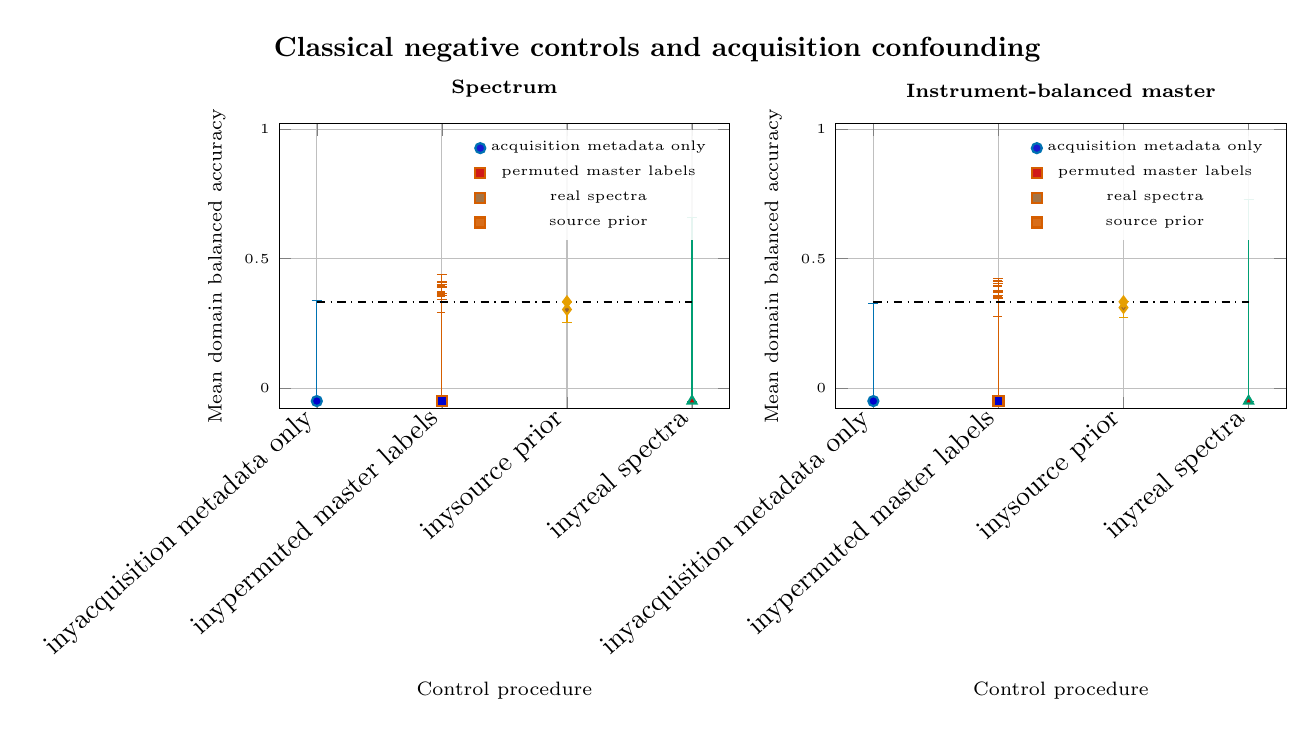
\begin{tikzpicture}
\begin{groupplot}[group style={group size=2 by 1, horizontal sep=1.35cm, vertical sep=1.5cm}, width=7.30cm, height=5.2cm, grid=major, tick label style={font=\tiny}, label style={font=\scriptsize}, title style={font=\scriptsize\bfseries,align=center}, legend style={font=\tiny,draw=none,fill=white,fill opacity=0.9,text opacity=1}]
\nextgroupplot[title={Spectrum},xlabel={Control procedure},ylabel={Mean domain balanced accuracy},ymin=-0.08,ymax=1.02,xtick={0,1,2,3},xticklabels={acquisition metadata only,permuted master labels,source prior,real spectra},x tick label style={rotate=42,anchor=east,font=	iny}]
\addplot+[color=atlas0,mark=*,mark size=1.8pt,line width=0.8pt,only marks,error bars/.cd,y dir=both,y explicit] coordinates {(0,-0.05) += (0,0.38899905) -= (0,0)};
\addlegendentry{acquisition metadata only}
\addplot+[color=atlas1,mark=square*,mark size=1.8pt,line width=0.8pt,only marks,error bars/.cd,y dir=both,y explicit] coordinates {(1,-0.05) += (0,0.43830107) -= (0,0)};
\addlegendentry{permuted master labels}
\addplot+[color=atlas1,mark=square*,mark size=1.8pt,line width=0.8pt,only marks,error bars/.cd,y dir=both,y explicit] coordinates {(1,-0.05) += (0,0.48701979) -= (0,0)};
\addplot+[color=atlas1,mark=square*,mark size=1.8pt,line width=0.8pt,only marks,error bars/.cd,y dir=both,y explicit] coordinates {(1,-0.05) += (0,0.40882513) -= (0,0)};
\addplot+[color=atlas1,mark=square*,mark size=1.8pt,line width=0.8pt,only marks,error bars/.cd,y dir=both,y explicit] coordinates {(1,-0.05) += (0,0.41410549) -= (0,0)};
\addplot+[color=atlas1,mark=square*,mark size=1.8pt,line width=0.8pt,only marks,error bars/.cd,y dir=both,y explicit] coordinates {(1,-0.05) += (0,0.4043655) -= (0,0)};
\addplot+[color=atlas1,mark=square*,mark size=1.8pt,line width=0.8pt,only marks,error bars/.cd,y dir=both,y explicit] coordinates {(1,-0.05) += (0,0.41047695) -= (0,0)};
\addplot+[color=atlas1,mark=square*,mark size=1.8pt,line width=0.8pt,only marks,error bars/.cd,y dir=both,y explicit] coordinates {(1,-0.05) += (0,0.41899928) -= (0,0)};
\addplot+[color=atlas1,mark=square*,mark size=1.8pt,line width=0.8pt,only marks,error bars/.cd,y dir=both,y explicit] coordinates {(1,-0.05) += (0,0.44309138) -= (0,0)};
\addplot+[color=atlas1,mark=square*,mark size=1.8pt,line width=0.8pt,only marks,error bars/.cd,y dir=both,y explicit] coordinates {(1,-0.05) += (0,0.44558019) -= (0,0)};
\addplot+[color=atlas1,mark=square*,mark size=1.8pt,line width=0.8pt,only marks,error bars/.cd,y dir=both,y explicit] coordinates {(1,-0.05) += (0,0.39224506) -= (0,0)};
\addplot+[color=atlas1,mark=square*,mark size=1.8pt,line width=0.8pt,only marks,error bars/.cd,y dir=both,y explicit] coordinates {(1,-0.05) += (0,0.4570019) -= (0,0)};
\addplot+[color=atlas1,mark=square*,mark size=1.8pt,line width=0.8pt,only marks,error bars/.cd,y dir=both,y explicit] coordinates {(1,-0.05) += (0,0.4419031) -= (0,0)};
\addplot+[color=atlas1,mark=square*,mark size=1.8pt,line width=0.8pt,only marks,error bars/.cd,y dir=both,y explicit] coordinates {(1,-0.05) += (0,0.46203853) -= (0,0)};
\addplot+[color=atlas1,mark=square*,mark size=1.8pt,line width=0.8pt,only marks,error bars/.cd,y dir=both,y explicit] coordinates {(1,-0.05) += (0,0.40883851) -= (0,0)};
\addplot+[color=atlas1,mark=square*,mark size=1.8pt,line width=0.8pt,only marks,error bars/.cd,y dir=both,y explicit] coordinates {(1,-0.05) += (0,0.42454153) -= (0,0)};
\addplot+[color=atlas1,mark=square*,mark size=1.8pt,line width=0.8pt,only marks,error bars/.cd,y dir=both,y explicit] coordinates {(1,-0.05) += (0,0.34152114) -= (0,0)};
\addplot+[color=atlas1,mark=square*,mark size=1.8pt,line width=0.8pt,only marks,error bars/.cd,y dir=both,y explicit] coordinates {(1,-0.05) += (0,0.43742835) -= (0,0)};
\addplot+[color=atlas1,mark=square*,mark size=1.8pt,line width=0.8pt,only marks,error bars/.cd,y dir=both,y explicit] coordinates {(1,-0.05) += (0,0.41863712) -= (0,0)};
\addplot+[color=atlas1,mark=square*,mark size=1.8pt,line width=0.8pt,only marks,error bars/.cd,y dir=both,y explicit] coordinates {(1,-0.05) += (0,0.40876373) -= (0,0)};
\addplot+[color=atlas1,mark=square*,mark size=1.8pt,line width=0.8pt,only marks,error bars/.cd,y dir=both,y explicit] coordinates {(1,-0.05) += (0,0.45104611) -= (0,0)};
\addplot+[color=atlas2,mark=triangle*,mark size=1.8pt,line width=0.8pt,only marks,error bars/.cd,y dir=both,y explicit] coordinates {(3,-0.05) += (0,0.70921614) -= (0,0)};
\addlegendentry{real spectra}
\addplot+[color=atlas3,mark=diamond*,mark size=1.8pt,line width=0.8pt,only marks,error bars/.cd,y dir=both,y explicit] coordinates {(2,0.30353866) += (0,0.026584278) -= (0,0.049955151)};
\addlegendentry{source prior}
\addplot+[color=atlas3,mark=diamond*,mark size=1.8pt,line width=0.8pt,only marks,error bars/.cd,y dir=both,y explicit] coordinates {(2,0.33333333) += (0,0) -= (0,0)};
\addplot[black,dashdotted,line width=0.7pt,forget plot] coordinates {(0,0.33333333) (3,0.33333333)};
\nextgroupplot[title={Instrument-balanced master},xlabel={Control procedure},ylabel={Mean domain balanced accuracy},ymin=-0.08,ymax=1.02,xtick={0,1,2,3},xticklabels={acquisition metadata only,permuted master labels,source prior,real spectra},x tick label style={rotate=42,anchor=east,font=	iny}]
\addplot+[color=atlas0,mark=*,mark size=1.8pt,line width=0.8pt,only marks,error bars/.cd,y dir=both,y explicit] coordinates {(0,-0.05) += (0,0.37724868) -= (0,0)};
\addlegendentry{acquisition metadata only}
\addplot+[color=atlas1,mark=square*,mark size=1.8pt,line width=0.8pt,only marks,error bars/.cd,y dir=both,y explicit] coordinates {(1,-0.05) += (0,0.45277076) -= (0,0)};
\addlegendentry{permuted master labels}
\addplot+[color=atlas1,mark=square*,mark size=1.8pt,line width=0.8pt,only marks,error bars/.cd,y dir=both,y explicit] coordinates {(1,-0.05) += (0,0.47454305) -= (0,0)};
\addplot+[color=atlas1,mark=square*,mark size=1.8pt,line width=0.8pt,only marks,error bars/.cd,y dir=both,y explicit] coordinates {(1,-0.05) += (0,0.39993247) -= (0,0)};
\addplot+[color=atlas1,mark=square*,mark size=1.8pt,line width=0.8pt,only marks,error bars/.cd,y dir=both,y explicit] coordinates {(1,-0.05) += (0,0.40839808) -= (0,0)};
\addplot+[color=atlas1,mark=square*,mark size=1.8pt,line width=0.8pt,only marks,error bars/.cd,y dir=both,y explicit] coordinates {(1,-0.05) += (0,0.40585979) -= (0,0)};
\addplot+[color=atlas1,mark=square*,mark size=1.8pt,line width=0.8pt,only marks,error bars/.cd,y dir=both,y explicit] coordinates {(1,-0.05) += (0,0.42842593) -= (0,0)};
\addplot+[color=atlas1,mark=square*,mark size=1.8pt,line width=0.8pt,only marks,error bars/.cd,y dir=both,y explicit] coordinates {(1,-0.05) += (0,0.39924242) -= (0,0)};
\addplot+[color=atlas1,mark=square*,mark size=1.8pt,line width=0.8pt,only marks,error bars/.cd,y dir=both,y explicit] coordinates {(1,-0.05) += (0,0.44611685) -= (0,0)};
\addplot+[color=atlas1,mark=square*,mark size=1.8pt,line width=0.8pt,only marks,error bars/.cd,y dir=both,y explicit] coordinates {(1,-0.05) += (0,0.46518258) -= (0,0)};
\addplot+[color=atlas1,mark=square*,mark size=1.8pt,line width=0.8pt,only marks,error bars/.cd,y dir=both,y explicit] coordinates {(1,-0.05) += (0,0.39496252) -= (0,0)};
\addplot+[color=atlas1,mark=square*,mark size=1.8pt,line width=0.8pt,only marks,error bars/.cd,y dir=both,y explicit] coordinates {(1,-0.05) += (0,0.46284873) -= (0,0)};
\addplot+[color=atlas1,mark=square*,mark size=1.8pt,line width=0.8pt,only marks,error bars/.cd,y dir=both,y explicit] coordinates {(1,-0.05) += (0,0.42539683) -= (0,0)};
\addplot+[color=atlas1,mark=square*,mark size=1.8pt,line width=0.8pt,only marks,error bars/.cd,y dir=both,y explicit] coordinates {(1,-0.05) += (0,0.46031006) -= (0,0)};
\addplot+[color=atlas1,mark=square*,mark size=1.8pt,line width=0.8pt,only marks,error bars/.cd,y dir=both,y explicit] coordinates {(1,-0.05) += (0,0.42106126) -= (0,0)};
\addplot+[color=atlas1,mark=square*,mark size=1.8pt,line width=0.8pt,only marks,error bars/.cd,y dir=both,y explicit] coordinates {(1,-0.05) += (0,0.41974607) -= (0,0)};
\addplot+[color=atlas1,mark=square*,mark size=1.8pt,line width=0.8pt,only marks,error bars/.cd,y dir=both,y explicit] coordinates {(1,-0.05) += (0,0.32760068) -= (0,0)};
\addplot+[color=atlas1,mark=square*,mark size=1.8pt,line width=0.8pt,only marks,error bars/.cd,y dir=both,y explicit] coordinates {(1,-0.05) += (0,0.44382716) -= (0,0)};
\addplot+[color=atlas1,mark=square*,mark size=1.8pt,line width=0.8pt,only marks,error bars/.cd,y dir=both,y explicit] coordinates {(1,-0.05) += (0,0.45398148) -= (0,0)};
\addplot+[color=atlas1,mark=square*,mark size=1.8pt,line width=0.8pt,only marks,error bars/.cd,y dir=both,y explicit] coordinates {(1,-0.05) += (0,0.41778199) -= (0,0)};
\addplot+[color=atlas1,mark=square*,mark size=1.8pt,line width=0.8pt,only marks,error bars/.cd,y dir=both,y explicit] coordinates {(1,-0.05) += (0,0.47477513) -= (0,0)};
\addplot+[color=atlas2,mark=triangle*,mark size=1.8pt,line width=0.8pt,only marks,error bars/.cd,y dir=both,y explicit] coordinates {(3,-0.05) += (0,0.77960317) -= (0,0)};
\addlegendentry{real spectra}
\addplot+[color=atlas3,mark=diamond*,mark size=1.8pt,line width=0.8pt,only marks,error bars/.cd,y dir=both,y explicit] coordinates {(2,0.31109594) += (0,0.022183742) -= (0,0.03981537)};
\addlegendentry{source prior}
\addplot+[color=atlas3,mark=diamond*,mark size=1.8pt,line width=0.8pt,only marks,error bars/.cd,y dir=both,y explicit] coordinates {(2,0.33333333) += (0,0) -= (0,0)};
\addplot[black,dashdotted,line width=0.7pt,forget plot] coordinates {(0,0.33333333) (3,0.33333333)};
\end{groupplot}
\node[font=\normalsize\bfseries,anchor=south] at (current bounding box.north) {Classical negative controls and acquisition confounding};
\end{tikzpicture}
\end{document}
